% !TEX root = ../main.tex
\chapter{Elaboration of the Workflow}
\label{chap:elaboration-of-the-workflow}

In this chapter I demonstrate the various steps of the static analysis workflow in detail. I employ small working source code examples in order to demonstrate the steps of the source code transformation. A prototype implementation of the proposed workflow is available as an open-source project at {\small\url{https://github.com/FTSRG/codemodel-rifle}}.

\section{Transforming the Source Code Into an AST}
As mentioned in~\Cref{sect:overview-transforming-the-source-code}, this transformation is carried out by the Shape Security Shift toolkit. The source code is passed to the parser along with the parameters for the parsing algorithm. Considering the new constructs introduced in ES6 (\Cref{sect:ecmascript}), I've chosen to parse every file as a \emph{Module}. This affects the grammar used in the parser and the resulting data model.
% TODO href Shift

The parse result of the one-line code snippet in~\Cref{lst:oneliner} was previously presented in~\Cref{fig:ast-asg-example}.

\begin{figure}[!htb]
	\begin{minipage}{\textwidth}
		\lstinputlisting[
			language=JavaScript,
			captionpos=b,
			caption={Basic example source code.},
			label={lst:oneliner},
		]{include/sources/oneliner.js}
	\end{minipage}
\end{figure}

\section{Storing the ASG in the Graph Database}
Once the source code is parsed and the ASG is returned, the framework updates the stored graph representation. Since \Cref{sect:maintaining-the-graph} details how the Java Object structure is transformed into a graph, this section only describes the queries used for the maintenance.

When a new file is added to the repository, there is no need to prepare the database. A new metadata node is created with the name and path of the file, and optionally the session identifier of the IDE it has been created and sent in to the framework. The subgraph representing the ASG is then inserted in a database transaction.

The newly created metadata node acts as a subgraph selector, since it is connected to every node belonging to the file (of the given session). This makes it easy to remove the file upon the removal of the file it represents.

In case the file has been modified, the nodes connected to its metadata node are removed, then the new graph is inserted.


\section{Division by Zero}
\label{sect:division-by-zero}
As one of the most basic and easy-to-discover mistakes, division by zero should be reported to the developer. In the context of mathematics, division by zero is undefined for the real numbers. In JavaScript, it may result in \code{NaN} or \code{Infinity}.

Without dynamic testing or symbolic execution it is rather hard to find this kind of expression, since the right side of the division may come from a variable. On the other hand, finding the cases where the right side is a literal is trivial.

Taking a look at~\Cref{fig:AST-PPT}, the graph representation of the previous example, it is relatively easy to find the problematic nodes. A natural language definition of the problem would sound like this: ,,we are looking for binary expressions that have a literal zero on the right side''.

\begin{figure}[!htb]
  \centering
  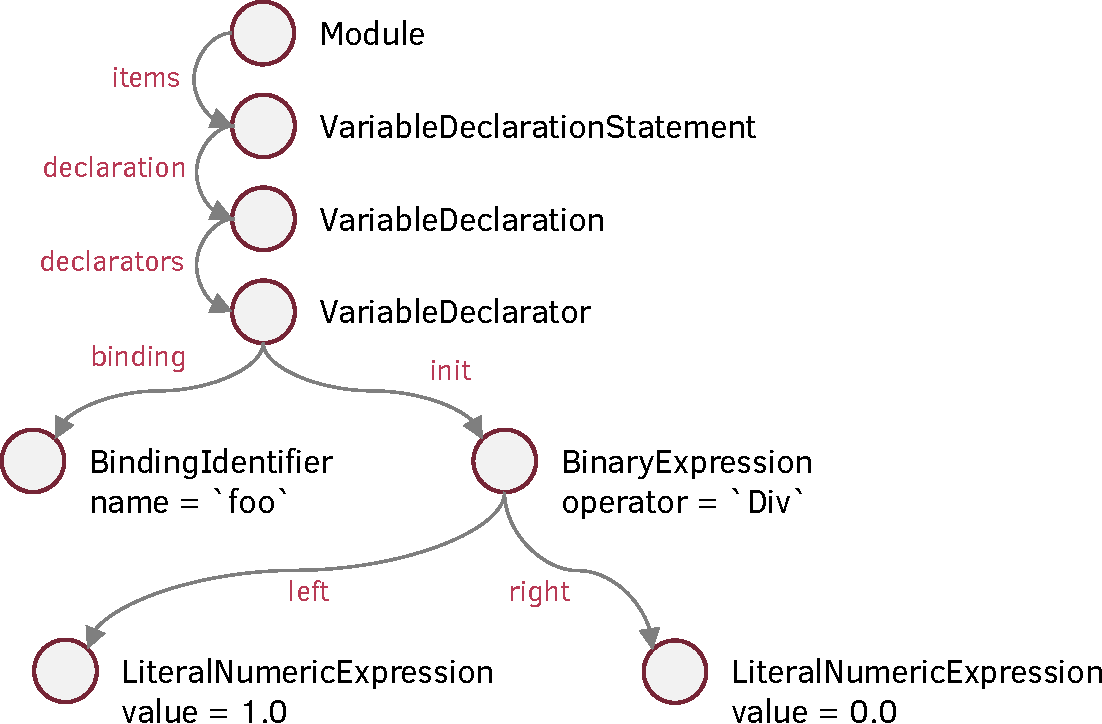
\includegraphics[width=0.8\textwidth]{AST-PPT.pdf}
  \caption{Graph representation of the code snippet of~\Cref{lst:oneliner}.}
  \label{fig:AST-PPT}
\end{figure}

One way to formalize this declarative definition in Cypher can be seen in~\Cref{lst:division-by-zero}. Executing this query on the AST of the source code would 1)~find matching nodes with the right type, 2)~bind them to the corresponding names, and 3)~check whether the required relations are present, resulting in a state like in~\Cref{fig:AST-query-PPT}. Finally, the result is the \code{BinaryExpression} node. By querying the source code location (also stored in the graph connected to the node) this query can report the precise location of the expression in the source code as problematic.

\begin{figure}[!htb]
	\begin{minipage}{\textwidth}
		\lstinputlisting[
			language=Cypher,
			captionpos=b,
			caption={Graph Pattern Matching Division by Zero.},
			label={lst:division-by-zero}
		]{include/sources/division-by-zero.cypher}
	\end{minipage}
\end{figure}

\begin{figure}[!htb]
  \centering
  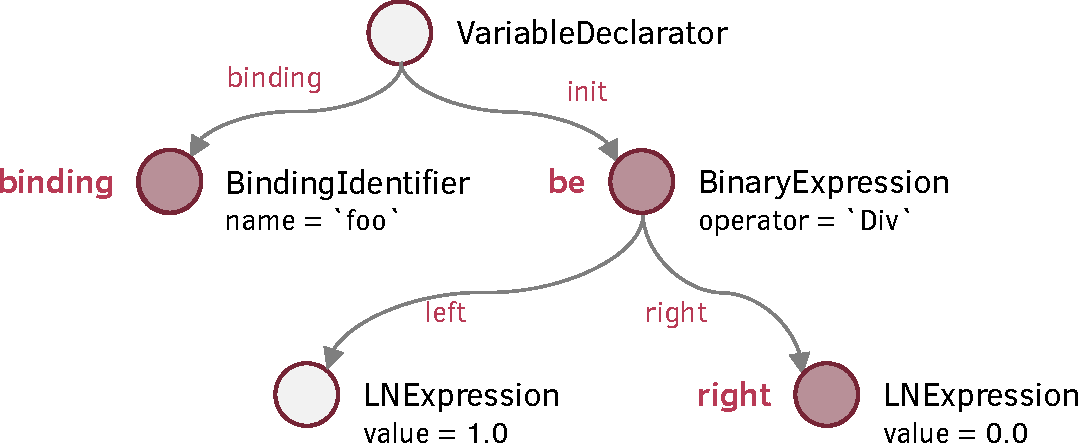
\includegraphics[width=0.8\textwidth]{AST-query-PPT.pdf}
  \caption{Graph representation of the query describing division by zero.}
  \label{fig:AST-query-PPT}
\end{figure}


\section{Handling Import and Export}
\label{sect:handling-import-export}
Since the beginning, JavaScript projects have grown tremendously. With the size of the average project, the language has also matured for handling bigger, more complex code repositories. With ES6, a module syntax has been introduced to spread the codebase into files, even directories. (Even before ES6 there have been several module systems, but ES6 described a standard for it.)

As described previously, I instruct the parser to process source files as modules. An ES6 \emph{module} differs in two ways from a \emph{script}: it is automatically interpreted as a \emph{strict-mode code}, and one can use \code{import} and \code{export} statements in them.

This section follows~\cite{ES6InDepth,ES6import,ES6export} and collects the most important details about the specifications.


\subsection{Export}
Everything declared inside a module belongs to the scope of the module. In order to let other modules to access them, they need to be explicitly exported.

\Cref{lst:es6-export} lists the various ways declaring a feature export. Just to list a few combinations; one may, for example, export expressions, variables, function and generator declaration statements either named, or using an alias. Or have default export expressions, even in an export statement.

\begin{figure}[htbp]
	\begin{minipage}{\textwidth}
		\lstinputlisting[
			language=JavaScript,
			captionpos=b,
			caption={ES6 export statement examples from MDN.},
			label={lst:es6-export},
		]{include/sources/es6-export-mdn.js}
	\end{minipage}
\end{figure}

Parsing these export statements result in different representation in the instance model and the resulting graph. \Cref{fig:es6-export-example} shows an example inline default export statement for a function named \code{foo}: \code{export default function foo() \{\}}. Note that the export statements are listed in the \code{Module}, but not in any of the \code{Scope}s.

\begin{figure}[htbp]
  \centering
  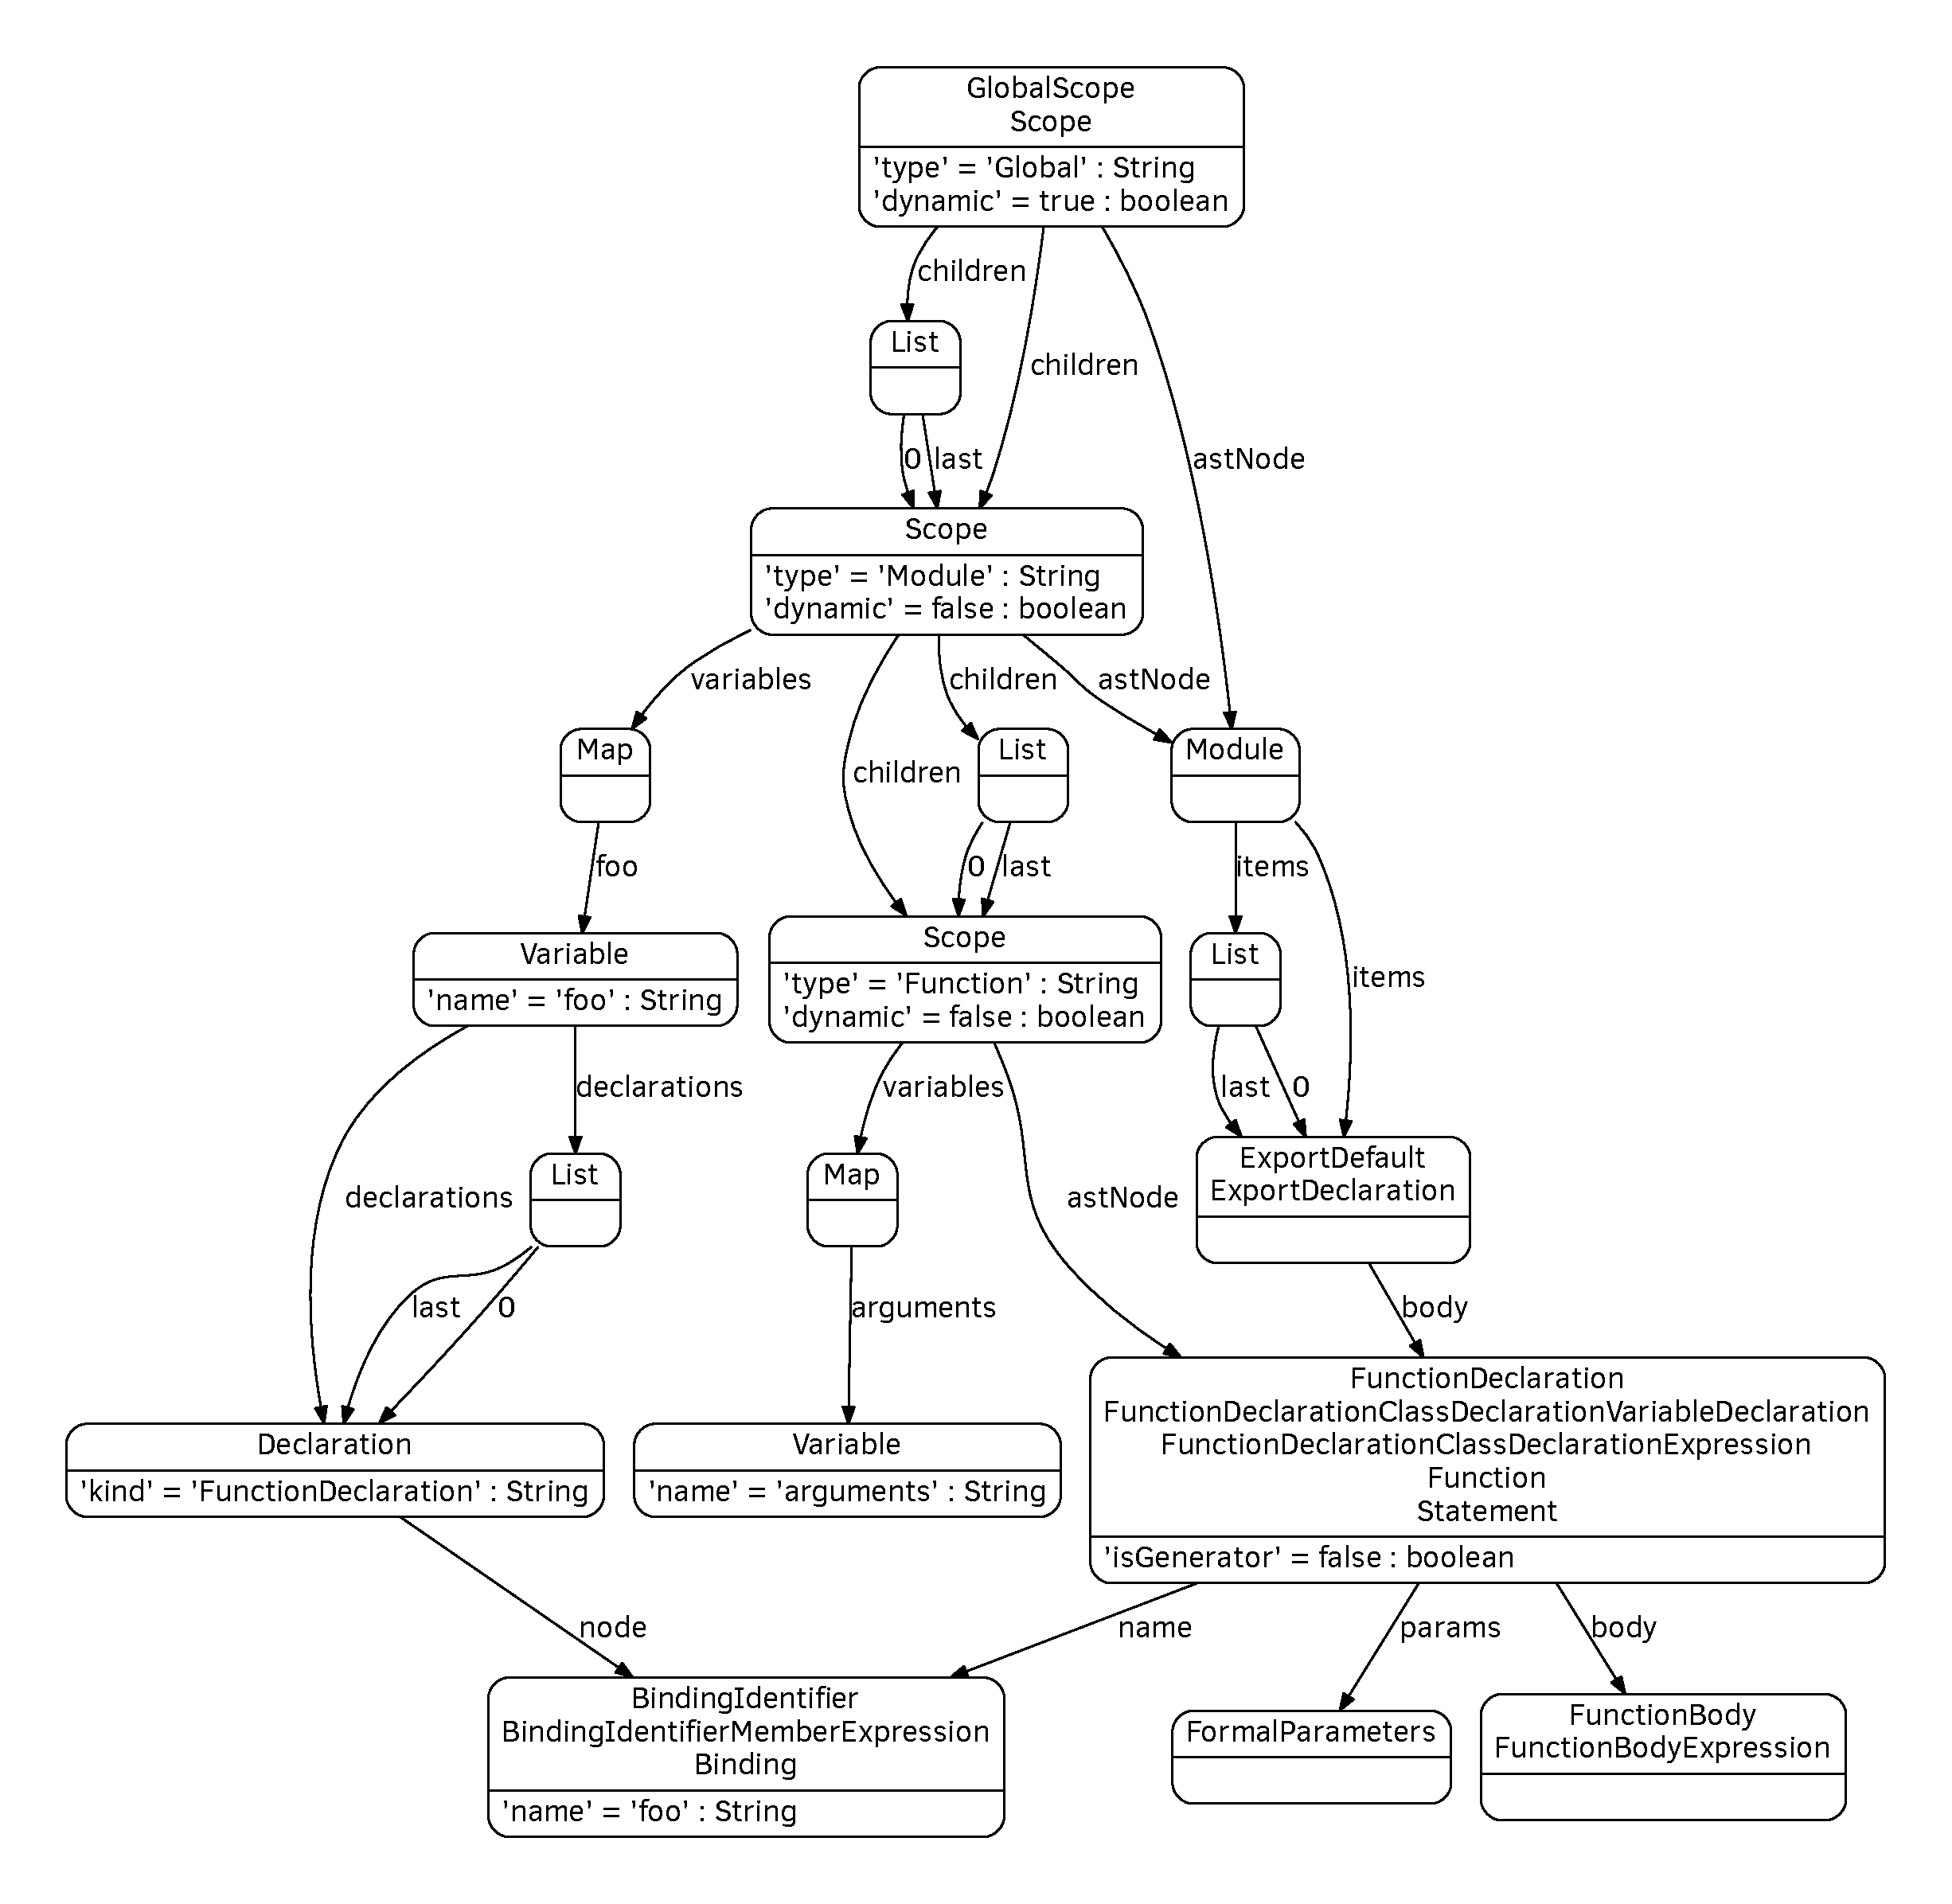
\includegraphics[width=\textwidth]{export-example}
  \caption{ES6 export statement example.}
  \label{fig:es6-export-example}
\end{figure}


\subsection{Import}
Like there are many ways for exporting features in a module, there are also several ways for importing them. \Cref{lst:es6-import} lists these.

\begin{figure}[htbp]
	\begin{minipage}{\textwidth}
		\lstinputlisting[
			language=JavaScript,
			captionpos=b,
			caption={ES6 import statement examples from MDN.},
			label={lst:es6-import},
		]{include/sources/es6-import-mdn.js}
	\end{minipage}
\end{figure}

The imported features are placed in the module-level global scope as a \code{Variable} without their declaring node, and the import statements are also present in the AST. \Cref{fig:es6-import-example} shows the ASG of a module importing and then using a function declaration (exported in the previous module): \code{import foo from "export"; foo();}.

\begin{figure}[htbp]
  \centering
  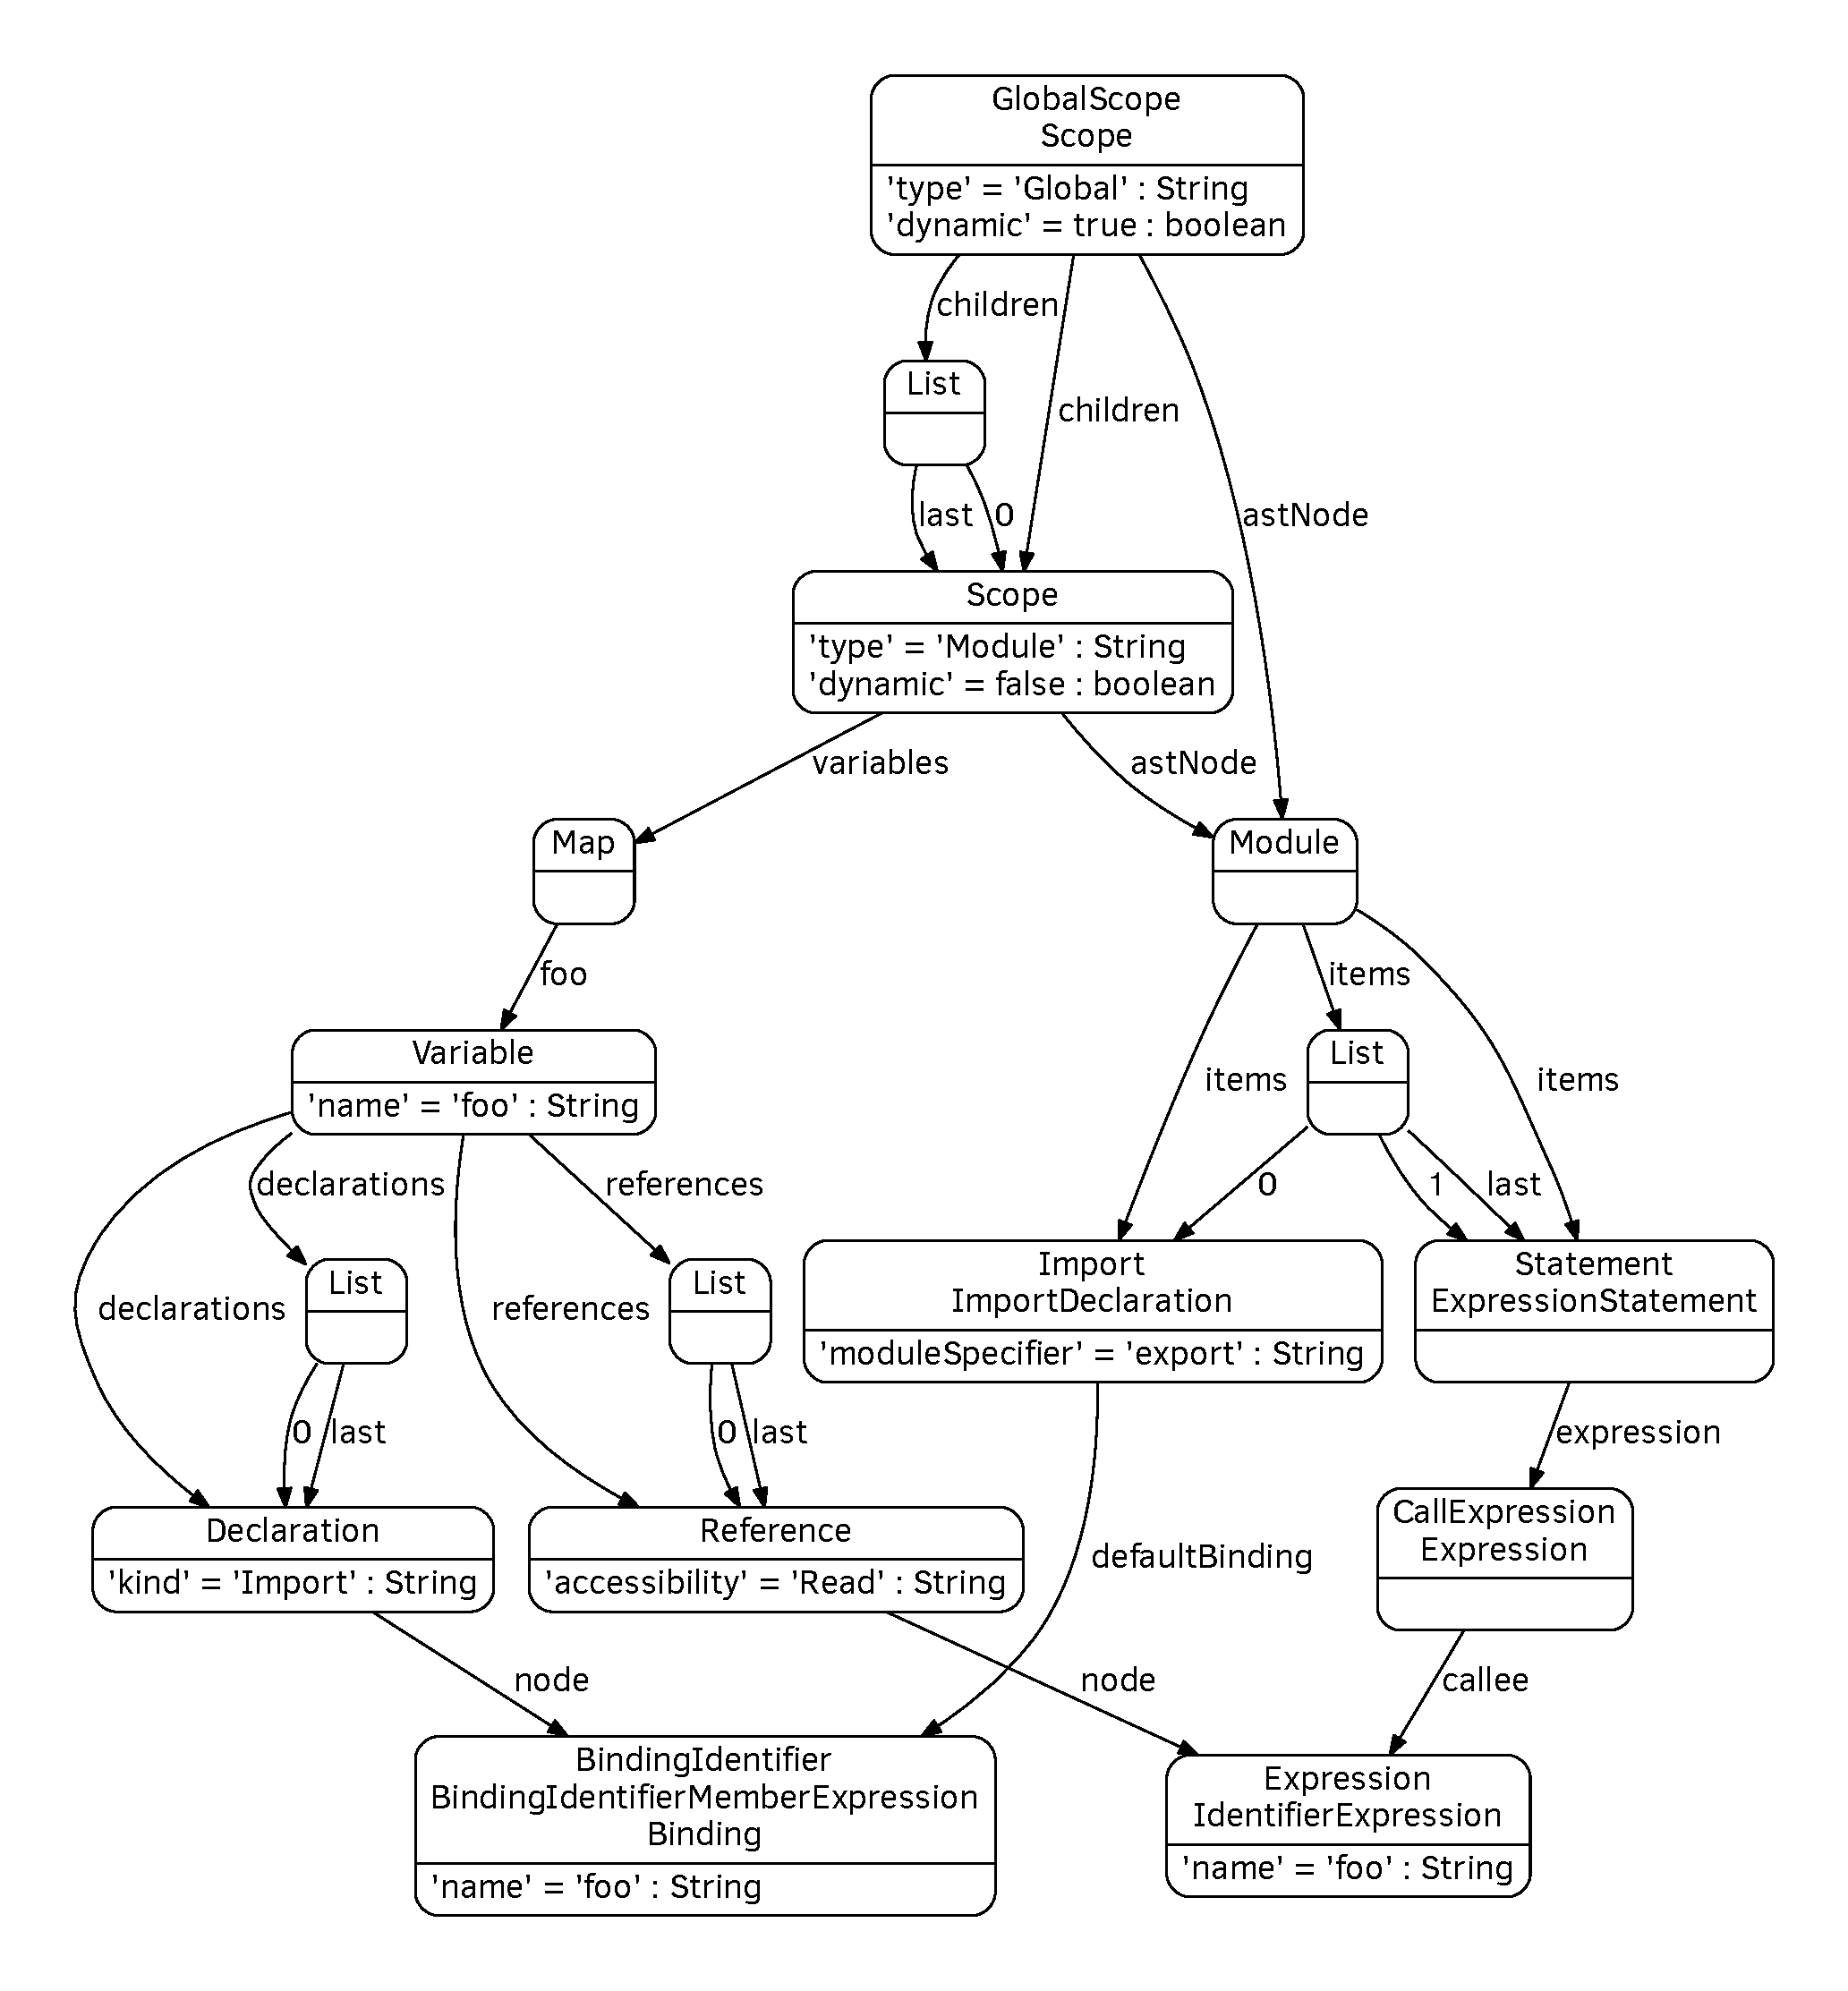
\includegraphics[width=\textwidth]{import-example}
  \caption{ES6 import statement example.}
  \label{fig:es6-import-example}
\end{figure}

\subsection{Connecting Imports to Exports}
Since there are several ways to both export and import features, there are even more combinations. This report does not aim to cover all of these, but to show that it is possible to connect graph module representations based on simple rules.

Executing the following steps emulates the resolution made by the interpreter of the source codes and connects the usages of the imported feature to the declaration of the exported one:

\begin{enumerate}[topsep=0pt]
	\item Find the imported \code{IdentifierExpression} in the \code{items} list of the \code{GlobalScope} node.
	\item Find the connected upstream \code{Variable} node.
	\item Find the \code{Declaration} for the \code{Export} that has a \code{Node} with the same \code{BindingIdentifier} as the import.
	\item Connect the \code{Variable} on the import side to the \code{Declaration} on the export side with a \code{declarations} relation.
\end{enumerate}

The Cypher query in~\Cref{lst:connect-import-export} manages to connect the exact type of imports and exports mentioned previously. Note that this query does not search for a file exporting the statement. For the correct match it should also check the metadata, whether the found node was declared in a file with matching absolute path.
% TODO absolute path

\begin{figure}[!htb]
	\begin{minipage}{\textwidth}
		\lstinputlisting[
			language=Cypher,
			captionpos=b,
			caption={Cypher query for connecting import and export statements.},
			label={lst:connect-import-export}
		]{include/sources/connect-import-export.cypher}
	\end{minipage}
\end{figure}

After executing the query in~\Cref{lst:connect-import-export}, the two ASG subgraphs are connected with a new edge (see~\Cref{fig:import-export-example}). This enables executing global-level queries addressing multiple modules. These newly added relations are always removed when either the source or the destination is removed, in case a module is modified. Thus it is optimal to run this query only when all of the files are already processed and the chance of modification in the near future is low. (This might happen after a modification is sent to the VCS or the developer saves the files in the IDE.)

\begin{sidewaysfigure}[htbp]
  \centering
  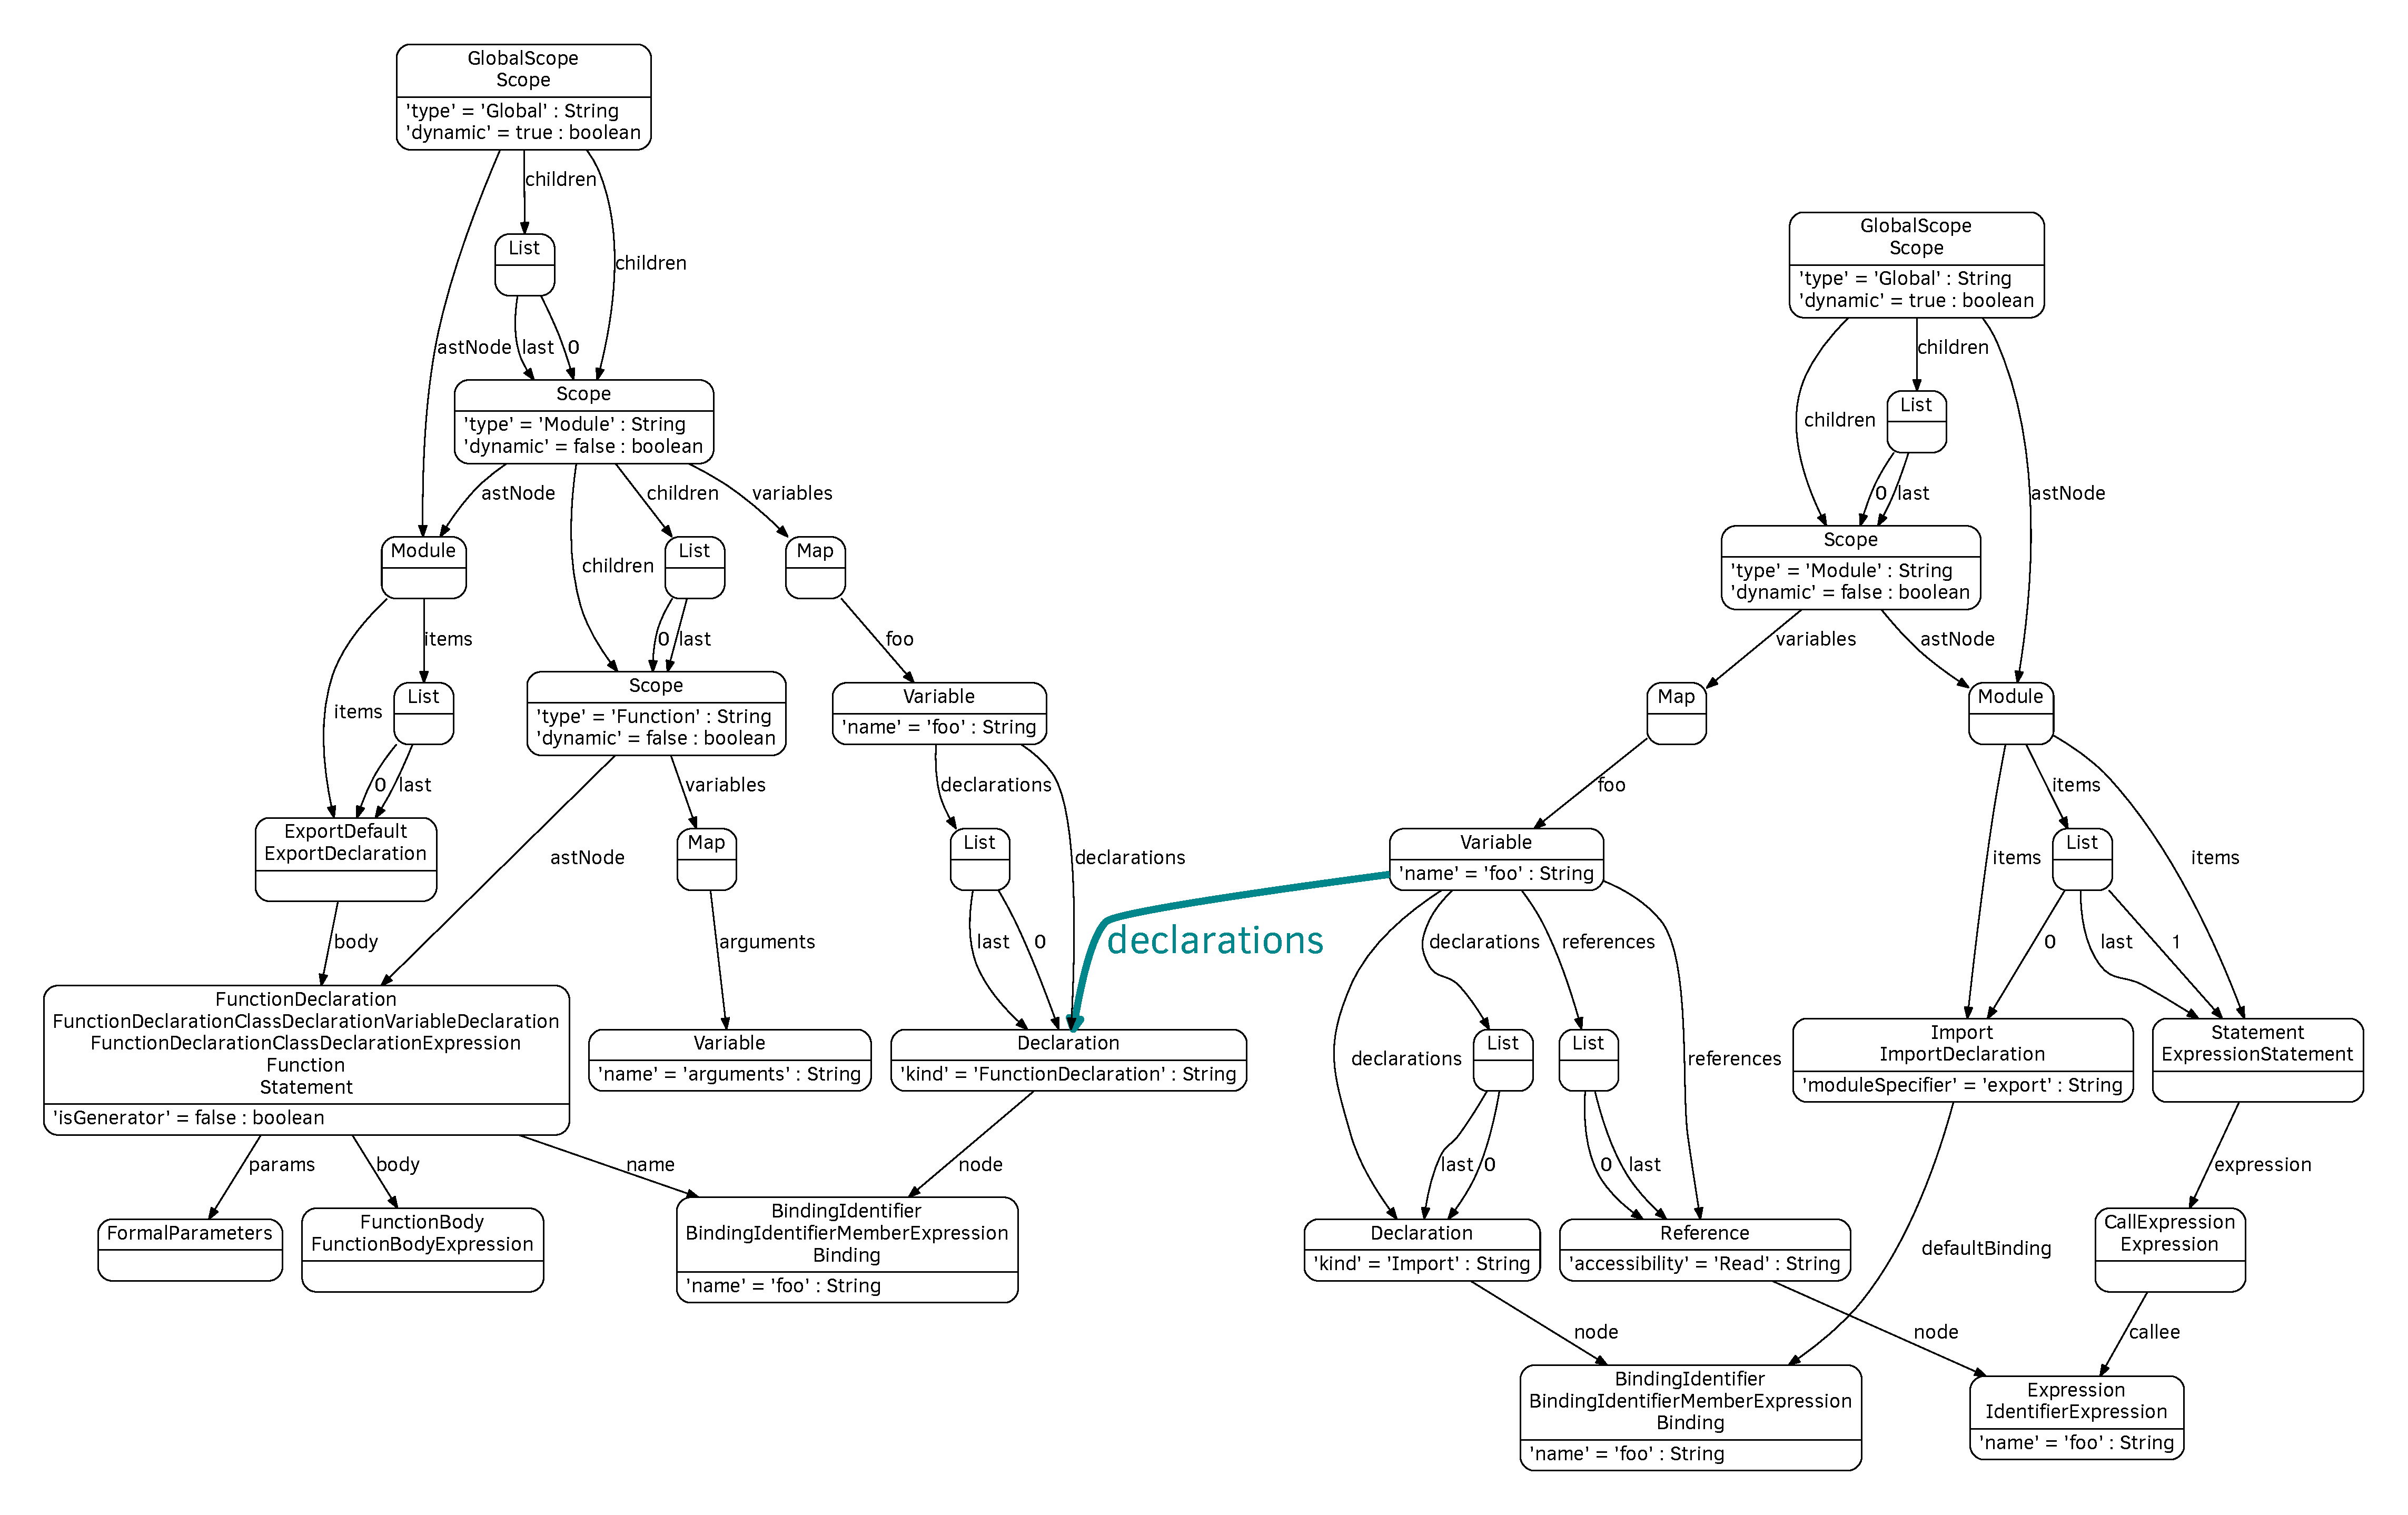
\includegraphics[width=\textwidth]{import-export-example}
  \caption{Connected ASG subgraphs.}
  \label{fig:import-export-example}
\end{sidewaysfigure}


\section{Dead Code Search}
\label{sect:dead-code-search}
Code that is written, but not used in the whole codebase is often called \emph{dead code}. Without symbolic execution it is a complex problem to decide what part of the code is reachable, but (excluding dynamic evaluation, e.g., \code{eval} in JavaScript) it is feasible to find function declarations in a file which are possibly not referenced in the local scope.
% TODO cite

\subsection{Search Algorithm as a Graph Query}
If a function declaration is not exported from the module and no exported declaration references it, it is highly likely that the declaration is unreachable and contains \emph{dead code}. With the following steps and the Cypher query described in~\Cref{lst:dead-code} it is possible to locate dead code in a file.

\begin{enumerate}
	\item Find the called \code{FunctionDeclaration}s target for every \code{CallExpression}.
	\item Find every call from the body of a function.
	\item Create a \code{calls} relationship between the caller and the callee \code{FunctionDeclaration}.
	\item Find the exported \code{FunctionDeclaration}s that can be entrance points.
	\item Find every \code{FunctionDeclaration} that should be available through the entrance points.
	\item Return every \code{FunctionDeclaration} that are not in this list.
\end{enumerate}

\begin{figure}[!htb]
	\begin{minipage}{\textwidth}
		\lstinputlisting[
			language=Cypher,
			captionpos=b,
			caption={Cypher queries for finding dead code.},
			label={lst:dead-code}
		]{include/sources/dead-code-search.cypher}
	\end{minipage}
\end{figure}

\subsection{Evaluating the Result}
For the sake of conciseness, I present the query for a simplified version of this algorithm, which only works with a single module in the database.

Compared to other commercially available software, this solution is able to detect more dead code scenarios: e.g., circular references without incoming calls (see~\Cref{fig:dead-code-result}. Instead of reporting the problems one-by-one or layer-by-layer, it reports the clique, without user input.

\begin{figure}[htbp]
  \centering
  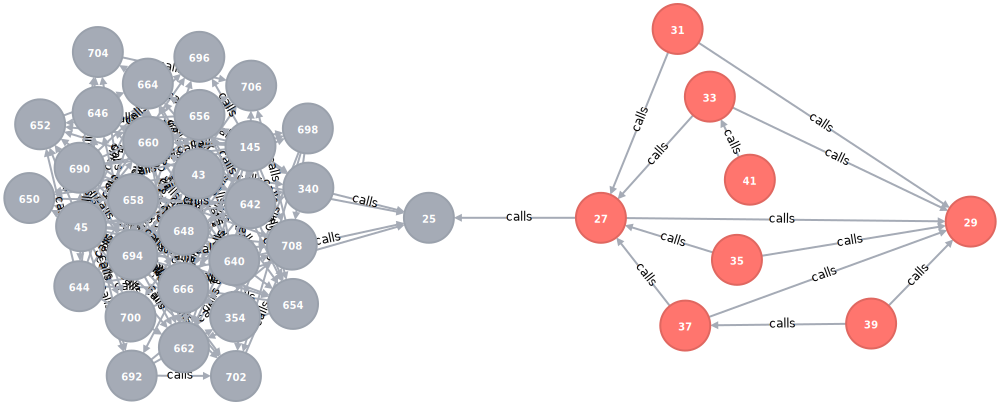
\includegraphics[width=\textwidth]{dead-code-result}
  \caption{Call graph with self-referencing clique in red.}
  \label{fig:dead-code-result}
\end{figure}
% TODO recolor and replace caption

\subsection{Transformation in a Transaction}
This query utilizes several possibilities only available in Neo4j. Since the query modifies the database, but the modifications are derived information, they should not be stored in the database. Database transactions that can be discarded, but still query the modified database are highly utilized here.

It is not possible to declare transitive closure\footnote{Transitive closure is marked with an asterisk in Cypher.} over arbitrary node type and edge label sequence in one Cypher query. This can be tackled by utilizing the \emph{trick} of starting a new transaction, writing the database and immediately querying the modified created data, then discarding the transaction. One can match and replace every sequence with a new, dedicated labeled edge and declare a transitive closure over it, but this requires the database to be modified (see~\Cref{fig:transitive-closure}).

\begin{figure}[htbp]
  \centering
  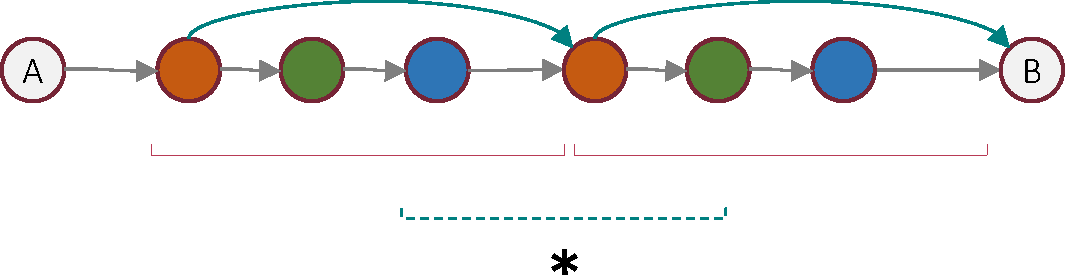
\includegraphics[width=\textwidth]{transitive-closure}
  \caption{Transitive closure over arbitrary node type and edge label sequence.}
  \label{fig:transitive-closure}
\end{figure}


\section{Control Flow Graph (CFG)}
\label{sect:transforming-asg-to-cfg}
Control Flow Graphs (CFG) are graph representations of the computation and control flows in the program. In this graph the nodes represent statements that are not interrupted by control changes. Directed edges represent possible flow of control between the two nodes. Nodes can have multiple incoming and outgoing edges.~\cite{IntroductionToCompilers}
\Cref{fig:CFG-PPT} presents an example CFG.

\begin{figure}[htbp]
  \centering
  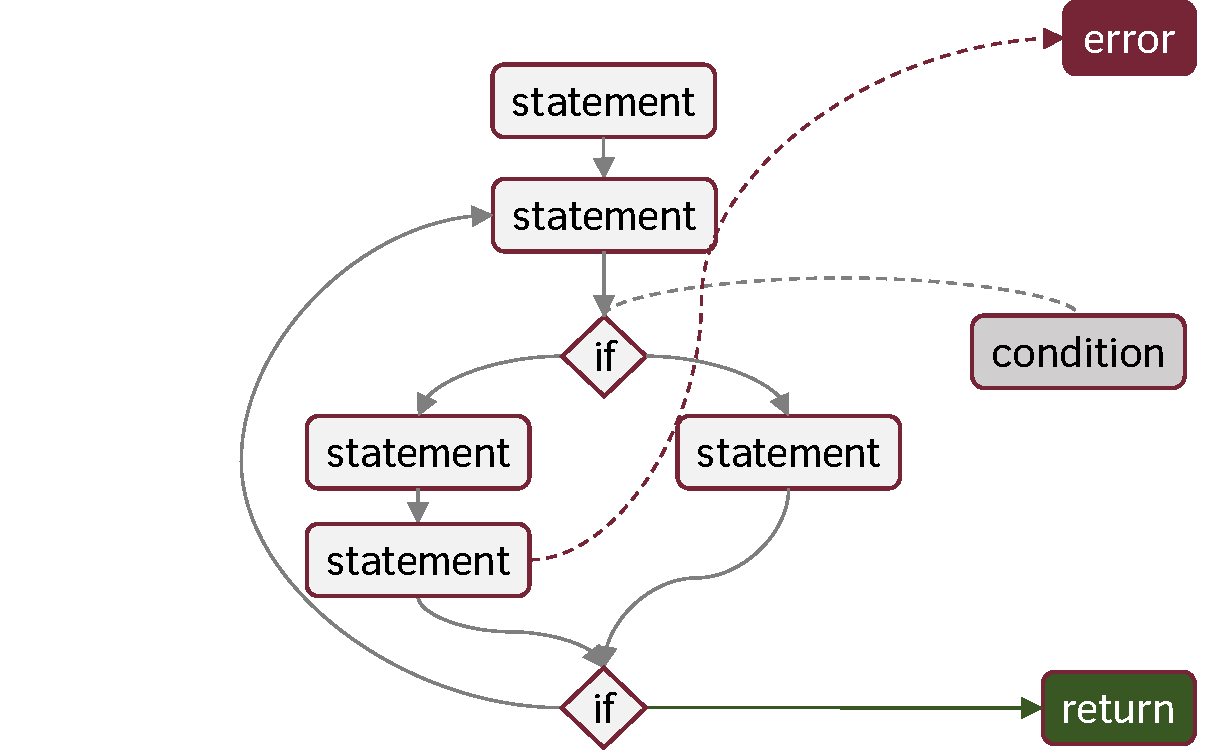
\includegraphics[width=0.75\textwidth]{CFG-PPT}
  \caption{Example control flow graph.}
  \label{fig:CFG-PPT}
\end{figure}
% TODO fix the CFG (if before return)

In this section I demonstrate how to transform the basic ASG structures into a CFG, and to utilize the result for static analysis.

\subsection{Theoretically Possible Paths}
\label{sect:cfg-paths}
As previously mentioned, nodes can have multiple incoming and outgoing edges. At execution time when the state of the program is at a given CFG node --- based on the dynamic state of the execution --- it may continue with any statement of the corresponding subsequent nodes.

Without running or interpreting the source code it is only possible to find and map every scenario in the ASG and transform them into nodes and edges in the CFG. A possible execution path is a path in the graph from one of the entry nodes to one of the exit nodes. The constraints on this path may be unsatisfiable, thus an execution of the source code may not iterate over this path. The CFG thus contains every feasible, and some infeasible execution paths.

\subsection{Transforming by Node Type}
There are several ways to transform the ASG into a CFG. Since my approach utilizes a graph database, the framework transforms the graph one smaller subgraph structure at a time, utilizing on pattern matching.

\subsubsection{Self-Containing Transformations}
% containing?
The key to this approach is widely used: every node has a \emph{start} and \emph{end} node that acts as a connection point for other nodes --- transformed at another time. These transformations will eventually connect the whole graph and represent the CFG.

This approach enables parallelization and thus speeds up the transformation, while generalizing the transformation patterns. The following sections present how different ASG information may be transformed.

\subsubsection{Sequencing}
Knowing the order of the statement sequences is one of the most important information for CFG transformations. Although it can be derived from the indexes of the list nodes, it is a rather compute-heavy operation. The graph thus redundantly contains the sequence information by storing the list elements both chained and indexed.

\subsubsection{Data Structures}
Data structures, like uninterrupted list of statements (statement blocks, such as the body of a function) may contain zero or more elements. Like previously detailed, lists are chained and the last element is also marked.

If the list contains one or more elements, the ASG structure is transformed as follows:
\begin{enumerate}[topsep=0pt]
	\item The \emph{start} node (the ASG node itself) is connected to the \emph{start} node of the first element.
	\item The \emph{end} node of every element except the last is connected to the \emph{start} node of the next element.
	\item The \emph{end} node of the \emph{end} node of the list itself.
\end{enumerate}

% TODO transformation figure

If the list does not contain any elements, its \emph{start} node is connected to its \emph{end} node.

\subsubsection{Statements}
As the main building blocks of a language, the various statement types represent different behaviors when interpreted. There are several statement types in the \emph{Shift} metamodel, and in this section I introduce a few of these for the purpose of building a small example program.

\paragraph{VariableDeclarationStatement}
A variable declaring statement is parsed into a structure of multiple graph nodes. These are \code{VariableDeclarationStatement}, \code{VariableDeclaration}, and \code{VariableDeclarator}. On the right side of the variable declaration statement is one \code{Expression}.

It is the framework's job to transform this ASG segment into a CFG. The transformation of any other element inside of the subtree of the root \code{VariableDeclarationStatement} node is executed at another time.

The assigned behavior to this node type and structure is the following:
\begin{enumerate}[topsep=0pt]
	\item The \code{Expression} is evaluated.
	\item The \code{VariableDeclaration} is executed.
\end{enumerate}

% TODO transformation figure

\paragraph{IfStatement}
This branching statement is parsed into one graph node. This node has two or three references. It must have one condition that decides the branching direction. A (positive) consequence is also required, but the alternate path reference is optional. In order to optimally transform these two scenarios, two transformation patterns are necessary.

\begin{enumerate}[topsep=0pt]
	\item Both scenarios evaluate the \code{Expression}.
	\item The positive consequence is connected with the \code{true} path, and the end node of the consequence node is connected to the end of the \code{IfStatement}.
	\item If there is an alternate branch, its start node is connected with the \code{false} path from the conditional \code{Expression} and its end node is also connected to the end node of the \code{IfStatement}.
\end{enumerate}

This transformation creates a diamond-shaped flow. If there are more alternative branches, the ASG represents them in chained containment. Thus eventually every branching will be connected, one-by-one.

\paragraph{FunctionDeclaration}
Function declaration structures are rather simple. The node has references to its parameters and body. The parameters --- if necessary --- are evaluated upon calling. The \code{FunctionBody} contains a list of directives and a list of statements.

The transformation pattern ignores the directives and immediately connects the \code{Function\-Declaration} to the list of \code{Statement}s, both ways (as after the function should also end after the last statement has been executed).

% BlockStatement
% ExpressionStatement

\subsubsection{Expressions}
There are 28 expression implementations in the Shift metamodel, for example literal expressions for strings, booleans, numerals, null, infinity, and regular expressions. There are also expressions representing class declarations, arrays, array functions. Unary and binary operators are also parsed into corresponding unary or binary expressions.

The prototype of the framework contains graph transformation patterns for literal and call expressions. Regarding the control flow graph, literals are immediately evaluated, so their end node is connected directly. Call expressions try to find the declaration of the called function and set it as the next block of the control flow.

The end node of the function declaration is also connected to the end node of the call expression. If the function is called more than once, its end node will have multiple outgoing edges. Thus when writing graph pattern queries over the CFG, one has to declare constraints matching the ingoing and outgoing edges between the \code{CallExpression} and the \code{FunctionDeclaration}.

In case the call expression provides parameters, they are also transformed into the CFG and evaluated in the given order.

\subsection{Transformation Challenges}
Besides the effort required for writing the transformation rules for every class and structure in the metamodel, there are also other challenges. Helping graph structures introduced for easy querying may slow down or even make impossible to correctly query given patterns.

Queries for dead code search (detailed in~\Cref{sect:dead-code-search}) for example require the list ordering and CFG end nodes to be removed, or the transitive closure slows down the query. This would make it unsuitable for near real-time user feedback.

Another challenge occurs, when a dynamic object or its member is passed as a parameter to a function call. When evaluated, the function declaration references it with an alias; the static analysis, however, may only guess the current value or reference. Substituting all the possible uses for a given reference and collecting dynamically added members may be a partial solution, but this is a future work of the research.

\subsection{Test Generation}
As previously mentioned in~\Cref{sect:cfg-paths}, the CFG contains every feasible, and some infeasible execution paths. In Cypher it is also possible to find the shortest paths or every path between two nodes. Knowing the entrance node of the CFG and selecting an arbitrary node in the CFG it is thus possible to list every path from the entry node to the selected one. This node can represent, e.g., a troublesome, unwanted or unexpected state.

With the transformation of the statements and the conditions of the if statements and other branching structures into a satisfactory problem it may be possible to decide whether there are program inputs that take the execution of the program to the selected node. This topic is subject to future work.


\section{Type Inference}
As detailed in \Cref{sect:introducing-type-inference}, type inference refers to the deduction of the data types of expressions, statements in the source code. My approach to finding the possible types of an expression or variable is similiar to the technique introduced in \Cref{sect:transforming-asg-to-cfg}, transforming the ASG into a CFG-like structure, as the data flow closely follows the control flow.

Type inference is a particularly difficult problem, even for statically typed languages. For dynamic languages, such as JavaScript, it is even more problematic and only a few tools are available. The most popular ones are listed in in \Cref{chap:related-work}.

Following the approach of one of these tools, Tern (introduced in~\Cref{sect:tern}), first I assign type information to given nodes in the ASG, then propagate this information based on constraints and rules, detailed in this section.

\subsection{Type System}
In order to represent the types in the graph, structures are introduced and stored in the same graph database. The database has a singular \code{TypeSystem} collector node, connected to every \code{Tag}, representing a type. These \code{Tag}s are attached to a given node, meaning the node can contain a value of the given type.

\subsubsection{Literal Types}
Since the literal expression nodes in the ASG are explicitly annotated with their type, it is the easiest to mark these nodes with a \code{Tag}: \code{Boolean}, \code{RegExp}, \code{Infinity}, \code{Numeric}, \code{Null}, and \code{String}.

\subsubsection{Classes}
Handling classes and composite structures requires new \code{Tag}s to be introduced to the type system. The \code{Tag}s should contain information about properties and methods, along with their possible types. The topic of developing the proper representation and transformations collecting and maintaining these structures is subject to future work.

\subsubsection{Functions}
Functions take parameters and based on inner logic (that could even consider the type of the parameters and other variables) may return any type of result. If the function declaration body returns a literal, an already tagged variable reference, or a new instance of a class, it is easily tagged.

The representation of function types is also subject to future work. I outline two possible representations:
\begin{enumerate}
	\item Maintain multiple type declarations for a given function, with every combination of parameter types.
	\item Store only a composite declaration with a list of possible values for every parameter and the return value.
\end{enumerate}

\subsection{Propagation Strategy}
As the program runs, the values and thus their respective types are moving from variable to variable through variable reads, operators, expressions, statements, and variable writes. While this process follows the control flow of the program, during static analysis there is no way to find the exact order of execution. Just like the CFG in my approach contains every possible flow, the type annotations in the graph will also contain every possible type that a given node may have.

The basic algorithm for propagating type information is the following:
\begin{enumerate}[topsep=0pt]
	\item Identify the literals and class instaces, tag these accordingly.
	\item Apply the propagation rules considering the constraints and propagate the tags so a given node can only have one reference to a given tag.
	\item Repeat step 2 until there is no modification in the graph --- or in case of an endless loop stop after given amount of iterations.
\end{enumerate}

\subsubsection{Expressions}
There are more than 25 types in the Shift metamodel for JavaScript. Some of these have discriminator values, that may result in different \emph{meaning} for different input types. \code{BinaryExpression}s have an \code{Expression} on their left and rigth side each with their type information, and the operator gives \emph{meaning} (semantics) to what the resulting value can be.

\Cref{table:addition-operator} shows the various semantics of a simple addition (a \code{BinaryExpression} with a \code{+} sign as a discriminating \code{BinaryOperator}).~\cite{js-arithmetic-operators}

\begin{table}[htbp!]
	\centering
	\begin{tabular}{lclclr}
		\toprule
		\textbf{Left expression} & \textbf{Operator} & \textbf{Right expression} & & \textbf{Result} & \textbf{Meaning} \\ \midrule
		Number                   &         +         & Number          & $\longrightarrow$ & Number  & \emph{(addition)} \\
		Boolean                  &         +         & Number          & $\longrightarrow$ & Number  & \emph{(addition)} \\
		Boolean                  &         +         & Boolean         & $\longrightarrow$ & Number  & \emph{(addition)} \\
		Number                   &         +         & String          & $\longrightarrow$ & String  & \emph{(concatenation)} \\
		String                   &         +         & Boolean         & $\longrightarrow$ & String  & \emph{(concatenation)} \\
		String                   &         +         & String          & $\longrightarrow$ & String  & \emph{(concatenation)} \\ \bottomrule
	\end{tabular}

	\caption{Semantics of the addition operator.}
	\label{table:addition-operator}
\end{table}

Logical operators also behave differently compared to other languages, e.g., Java. The logical and operator (\code{\&\&}) returns the left expression if it is so-called \emph{falsy} (values that can be converted to \code{false}, such as \code{null}, \code{0}, \code{undefined}). If the left side expression is \emph{truthy}, it returns the right side value. Thus the possible return \emph{type} of the expression can be types of both expression and not necessarily \code{Boolean}.

Apart from \code{UnaryExpression}s and \code{BinaryExpression}s, there are several more. Most importantly the \code{CallExpression}, that returns the value of the called function. A value with possible \emph{types} that the function may return with. Just like in case of the CFG transformations, several rules have to be written in order to cover the various expressions of the language.

Since the base of the transformation is the ASG, where the expression is parsed in the correct precedence, the transformation will also respect this order and compute the possible types of the whole expression.

\subsubsection{Statements}
There are also more than 20 \code{Statement} types in the metamodel of Shift. Some of these introduce new, temporary variables in the scope, such as \code{ForStatement} or its specific, \emph{syntactic sugar} version, \code{ForOfStatement}, that iterates over the values of an iterable type. In these cases the transforming graph pattern has to extract the inner type information from the type of the iterable and propagate it to the variable.

\subsubsection{Variable References}
In JavaScript one may think of a variable identifier as a label, a name, a reference to a value. These variables are represented in the ASG and (most of) their static access references are also represented.

When an \code{Expression} accesses the value of a \code{Variable}, a reading \code{Reference} is present in the ASG. The same goes for the \code{VariableDeclarationStatement}s and \code{ExpressionStatement}s with \code{AssignmentExpression} inside, assigning value to a variable, represented by a writing \code{Reference}.

These \code{Reference}s are only present for static scope variable accesses. New transformation rules have to be created to cover the cases when an \code{Object} is dynamically introduced to a scope --- e.g., passed as a parameter for a function. This is also subject to future work.

\Cref{fig:type-propagation} shows how the type information may propagate in the graph. After the \code{Literal}s have been tagged \circled{1}, the type information propagates to the \code{Variable} \circled{2} through the \code{VariableDeclarator} and the \code{BindingIdentifierMemberExpression}. This type information is read by the \code{IdentifierExpression} \circled{3} and the final type of the \code{BinaryExpression} based on the rules of adding a number to another number will be calculated and assigned \circled{4}.

\begin{figure}[htbp]
  \centering
  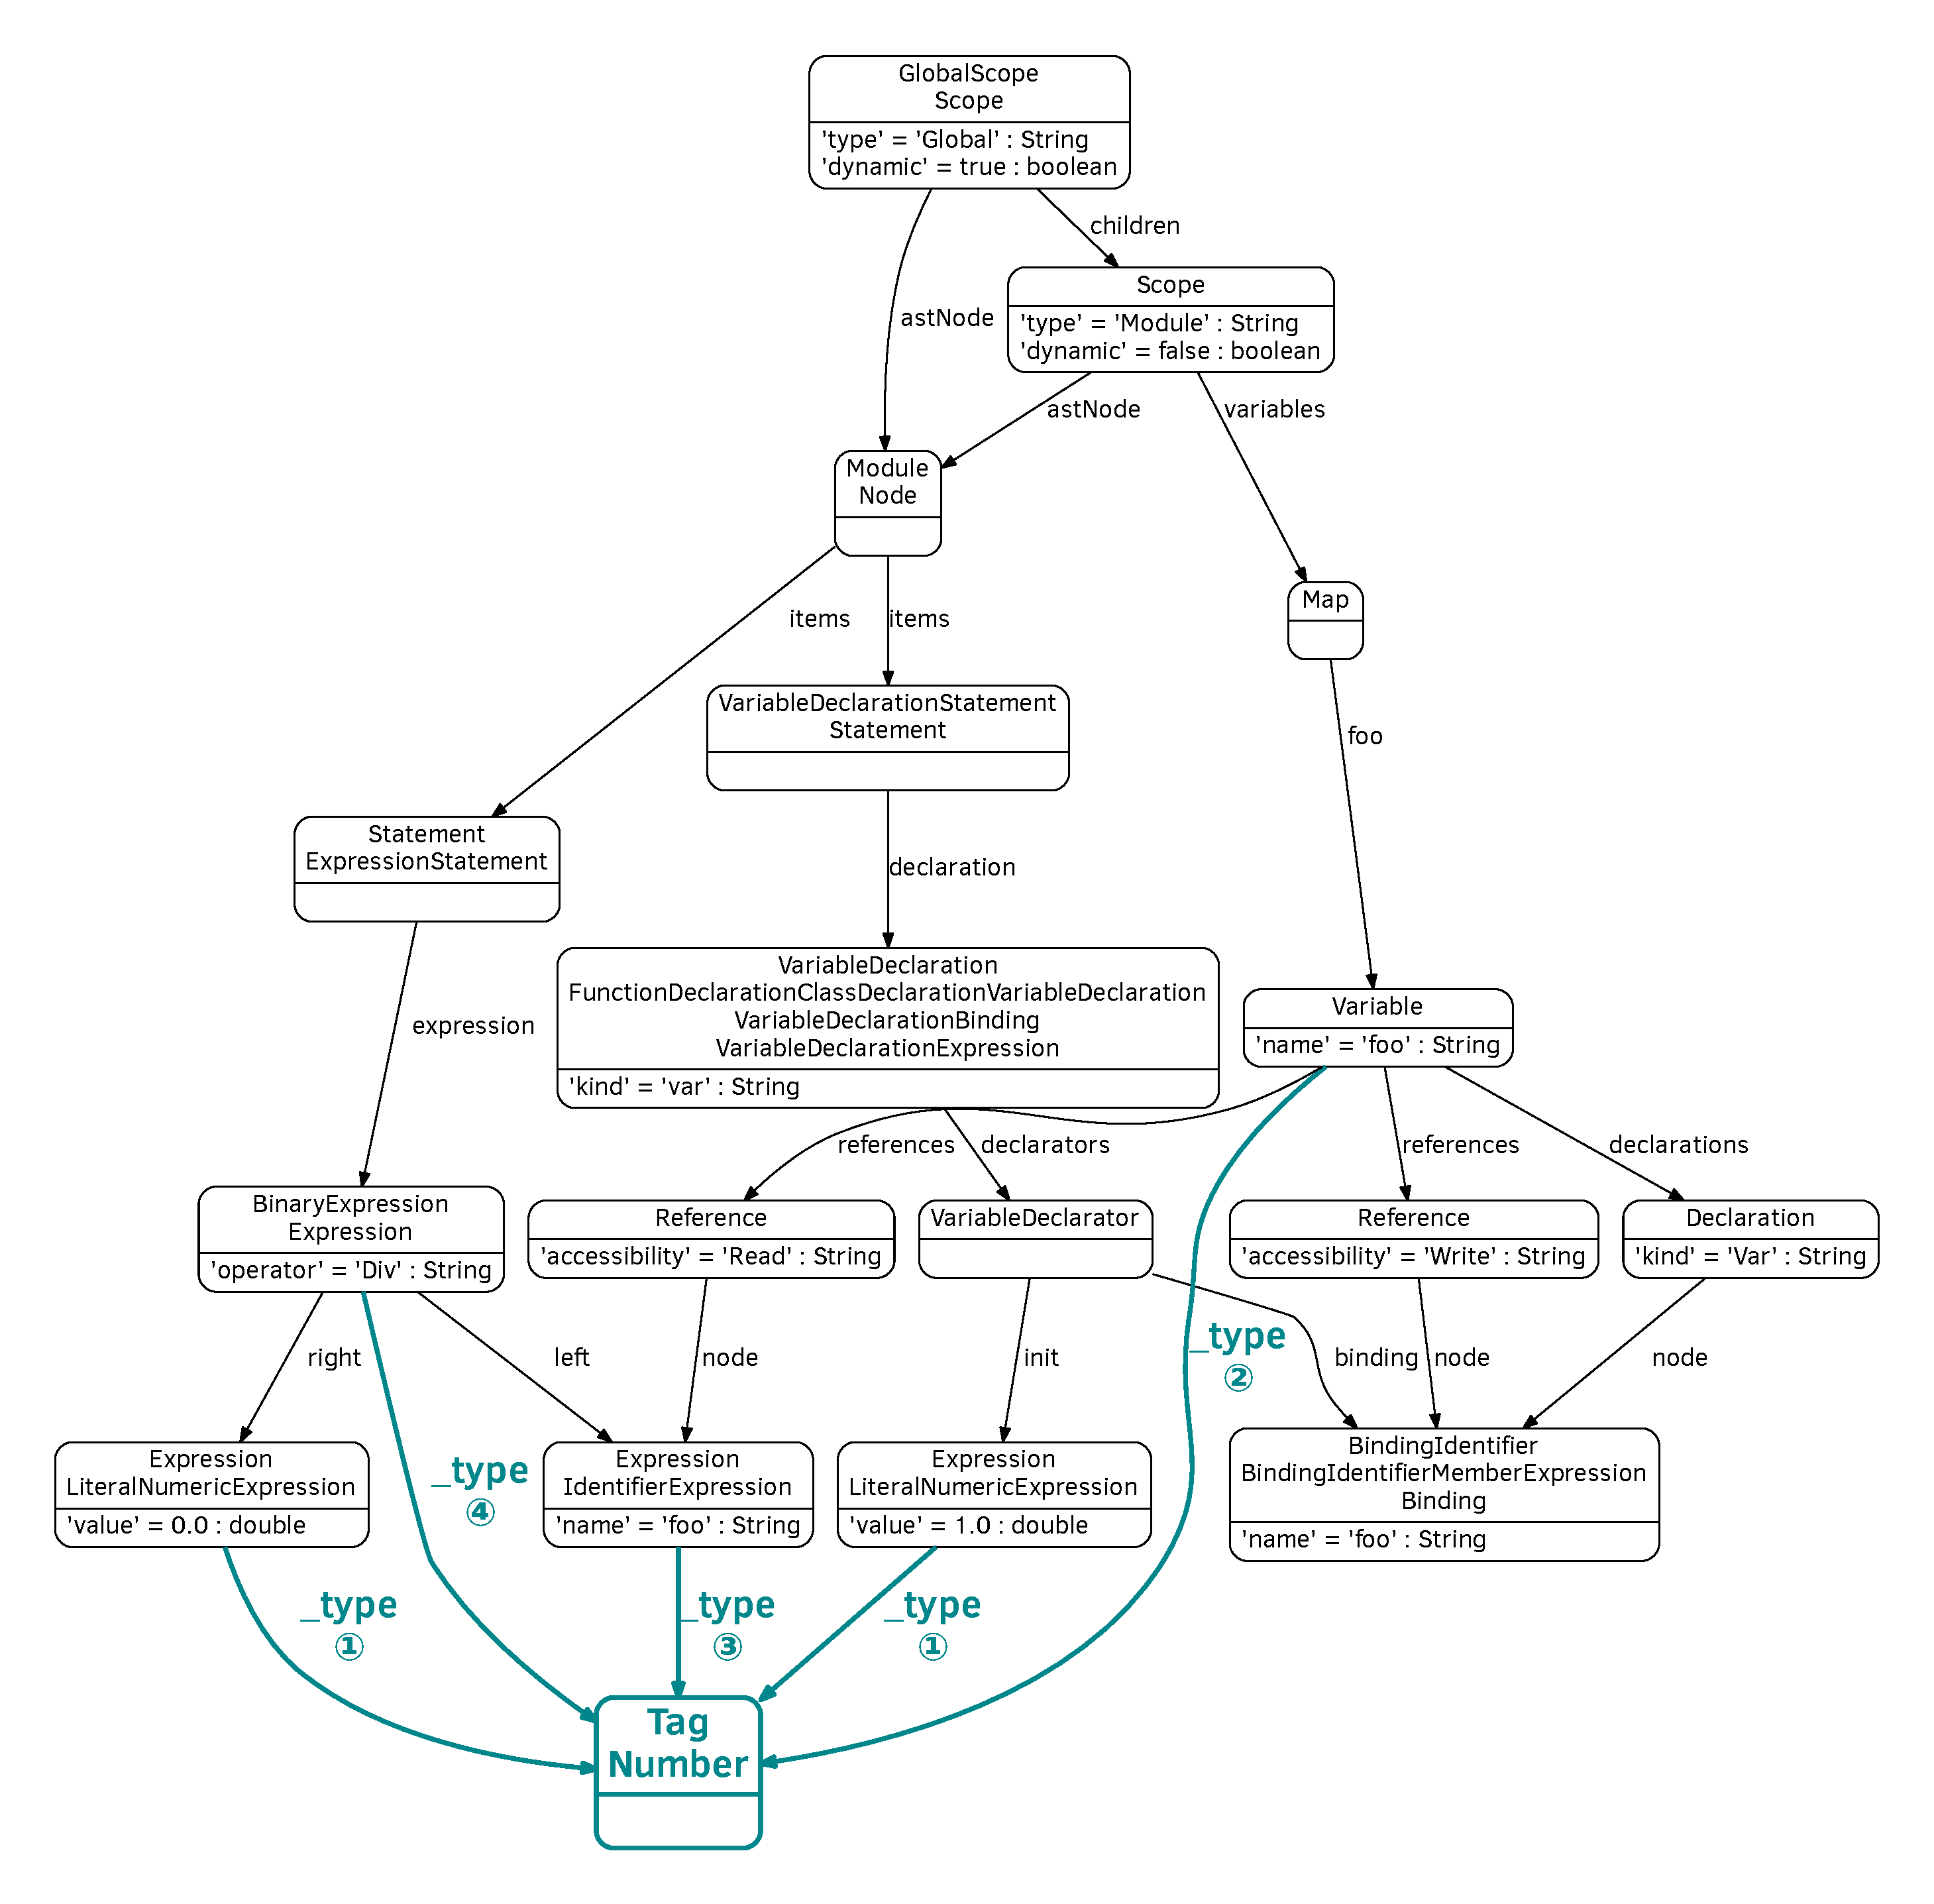
\includegraphics[width=\textwidth]{type-inference-steps}
  \caption{Type information propagation.}
  \label{fig:type-propagation}
\end{figure}

\subsection{Limitations and Challenges}
For my thesis I have only investigated whether it is possible to build the foundations of a type inferencing system on graph pattern matching and transformations. The type inferencing system in Tern (introduced in~\Cref{sect:tern}) has already shown that it is possible to do so on in-memory AST representations with visitor patterns.

In order to achieve better language coverage, it is subject to future work to develop an appropriate representation for compound and complex data structures, handle built-in functions and methods of data types. Challenges also include handling the \code{this} references in functions and class methods, anonymous functions, and method calls like \code{forEach}, \code{map}, or \code{filter}.

With the right constraints it is possible to approximately infer the type of a given expression and help developers with context-aware information and warnings for type-related problems.

%\section{Language Limitations}
% object as a parameter
% default parameters
% rest parameters (...)
% no evaluation
% only a small selection of language elements supported
% TODO write
